
\chapter{Project Management}
\label{cha:management}

\section{Development Methods}
\label{sec: development_methods}

We discussed the possible use of software engineering techniques we could utilise to make things easier and to ensure success and good planning. In a way it was hard, since we have no concrete experience about how much work a single software engineer can do and so forth.

\subsection{Weekly Meetings}
In the weekly meetings we discussed our progress so far on the whole project and any problems that had arisen on the week and how we could get around them and fix them. We went over our plans of what we would have to have done during the next week and revised if it still was a good idea and possible to implement at that stage. After deciding what we wanted to accomplish in the next week we tried to split the tasks evenly amongst us.
\\ \\
We usually had two meetings a week, one on Tuesday and one on Thursday with the demonstrator. After we got feedback from the demonstrator we reviewed our plans. Depending on what we discussed we usually wrote logs and drew some rough drafts about what to do. Our main communication medium has been Facebook. We formed a group there where we only have the members of our team and we have been dealing with assigning tasks over it and talking over any problems we might have. I have been quite surprised how well it has worked for a thing like this.

\subsection{Incremental Stages}
We decided to build the base game first, without anything fancy in it, as in the absolute core of the game. So we started out making the ships with just shapes and not sprites. After we got that to render properly, we started adding movement, opponents, spawning and shooting. \\\\
Basically we built the game in incremental stages, first making the core and then adding functionality on top of that. The goal was to have a working copy with more functionality at the end of every week, according to our schedule and plans. I think we managed that fairly well. At the very start we decided to try to keep the game at a bare minimum, no extra fancy stuff added or even planned very far until the core was working well, since we knew the hazards of getting stuck with planning and daydreaming without getting anything worthwhile working in the end.

\section{Planning}
\label{sec: planning}
We ended up with the idea of trying to document everything as well as we can and use weekly meetings to plan out the tasks for that week and where we want to be after it. So we set our iteration period to last a week and assigned tasks at the start of it. Requirements documentation and user requirements was among the things we knew are critical if you want a project to succeed in the timeline it has been given.\\\\
Trying our best to decide how much time to use on each part and how to divide the tasks in even portions, so that the contribution would be spread evenly amongst us. But as said above, we found it to be rather difficult since we had no clear concept of how hard it would be to code networking and other parts we had no experience about.\\\\
One thing that was a bit daunting was the team work itself, since no-one of us had any experience in it either, so how would it work if we had to work on a class that someone else was working on already and how to arrange it all so that it would not get too messy.
In the end we drew a rough diagram on how to organise our packages and classes and a basic timeline of when we would want each version to be out and what would it entail.

\section{Testing}
\label{sec: se_testing}
Testing is obviously and important part of any software development. At the very start of the project we decided to test everything well and throughly, if possible. We didn't have any experience with JUnit or testing in general, apart from the things we have done to debug our code and show testing with main methods during the first year.\\\\
After the lecture on testing and some help with the demonstrator we set up our tests and managed to test everything we had done so far and it all seemed to be in order. At the next stages of the project, I must admit, that we did not really utilise JUnit testing until the very end. But this does not mean we did not test everything. Everyone took care that the code they committed was tested with main methods and different kind of System.out.print commands.

\section{Time Management}
\label{sec: time_management}
When beginning the project, a time plan was created to provide detailing to ensure the project stayed on track and was completed on time. The Gantt chart for the project is shown below.
\begin{center}
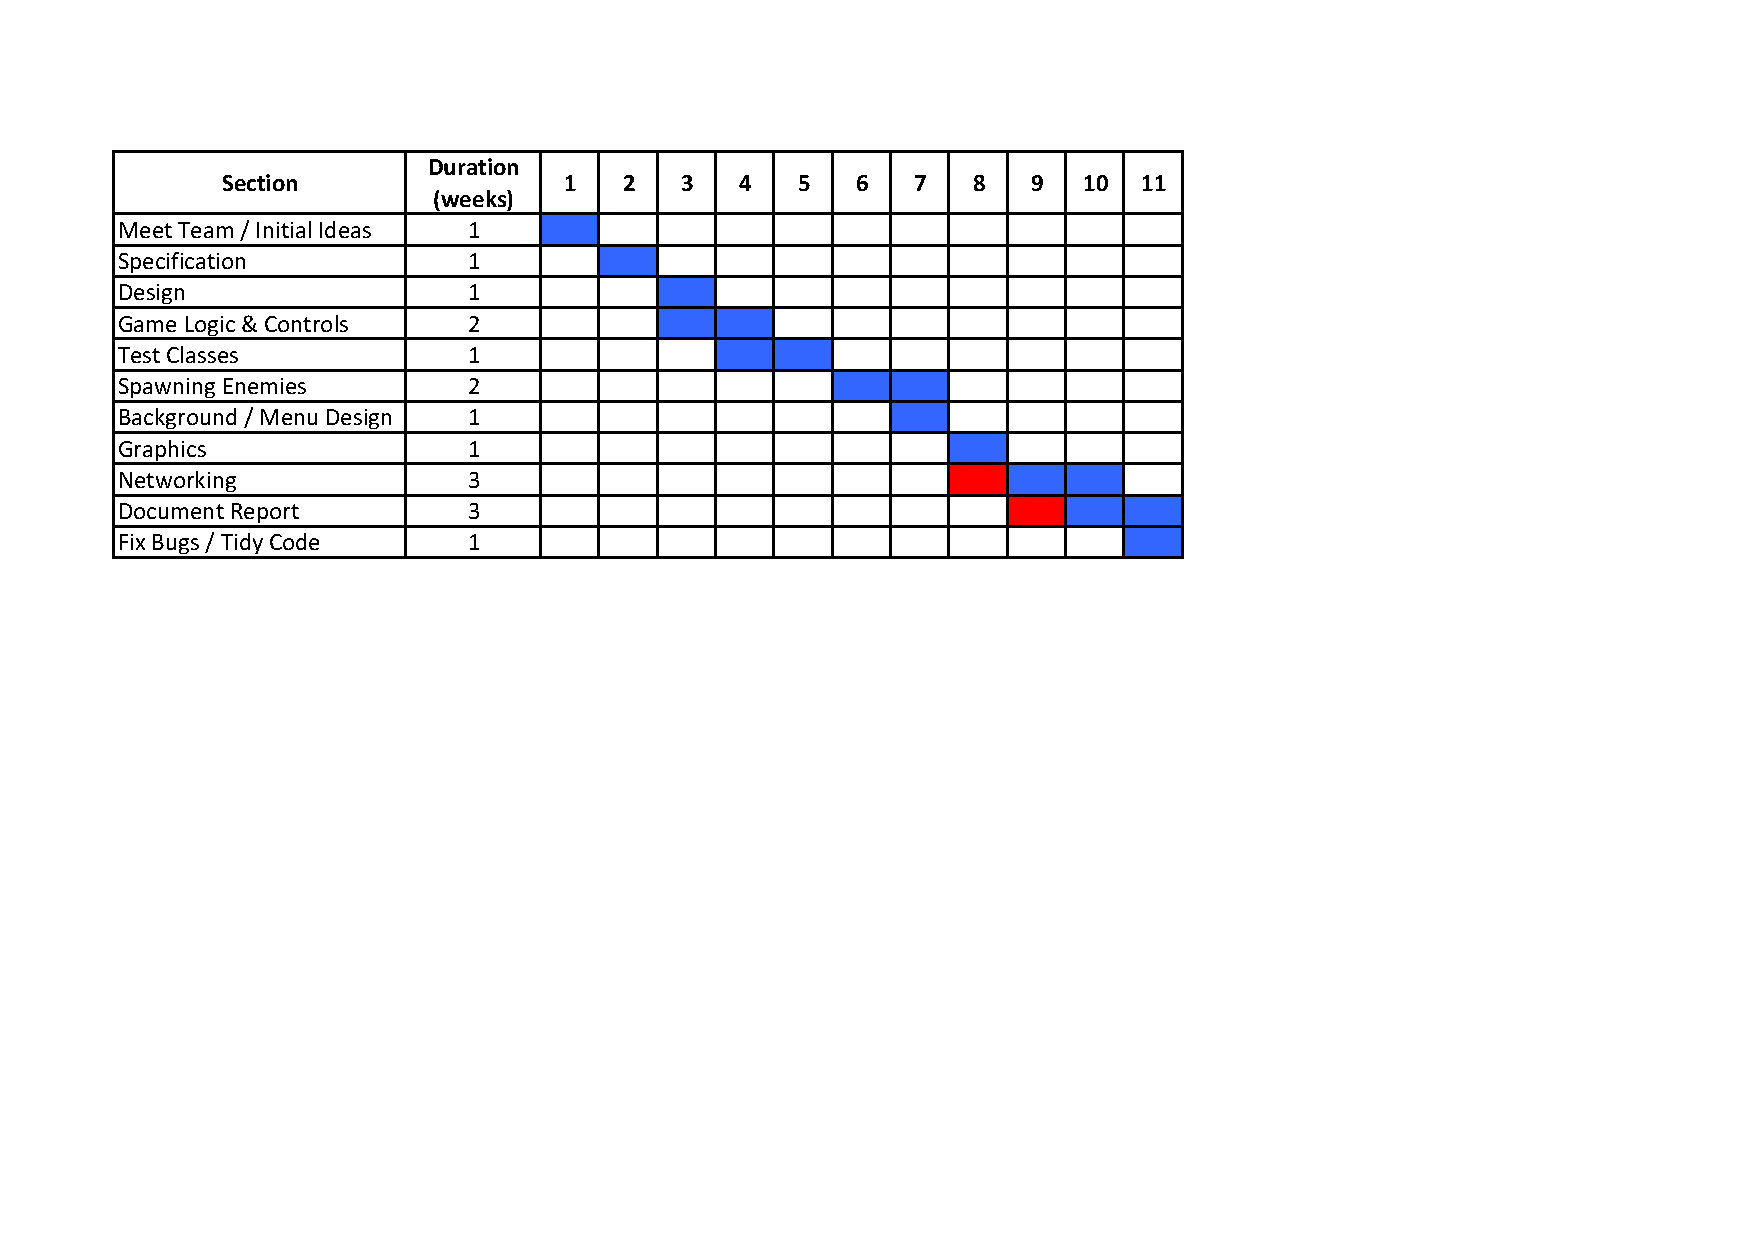
\includegraphics[width=16cm]{gantt.pdf}
\end{center}
The project was delayed slightly towards the end of the project which mean't it would become slightly rushed. However, the team managed to allocated appropriate resources to the sections that required more attention (networking) whilst the remainder of the team continued to work on the final report.\\\\
Overall, the project was delivered on-time and the coding introduced additional features which weren't in the initial requirements but documented in the future requirements.

